% !TEX root = proposal.tex
\section{Hypothesis} \label{sec:hypo} 

In this section, I discuss about hypotheses that we want to verify and confirm
from my thesis.

\subsection{\sreplica Generalization}

Even though, our previous work most focuses on a specific instance of inline
monitor (\ie DFT), we strongly believe that the approaches can easily be
generalized to support analyses of other kinds only with minimal amount of
effort.  Tabel~\ref{tab:analyses} contains a list of well-known inline
monitors~\cite{CAB} echo one's goal is either to protect or profile application
processes dynamically. Column entries categorizes monitors according to its
structural properties. Column entry {\it Shadow Memory} denotes whether the
monitor requires shadow memory area to keep track of updates from real
execution context. {\it Data dependency} denotes whether the monitor's
operations depend on it own previous updates. We have to consider data
dependencies between updates if we want to parallel the analysis performed by
the monitor. {\it Check Operation} denotes whether the monitor examines for
specific system activities. For instance, DTA tool checks for every {\tt RET}
structions to see whether a taintedness value is used for its operand to
deviate executions. In contrast, {\it cache simulation} does not have such
operations.

\begin{table}[h]
    \centering
\begin{tabular}{|c|c|c|c|}
\hline
Analyses & Shadow Memory & Data Dependency & Check Operation \\ 
\hline \hline
Data Flow Tracking (DFT) & O & O & O \\ \hline
Control Flow Integrity (CFI) & O & O & O \\ \hline
\specialcell{Memory Integrity Tool \\ (Memcheck)} & O & O & O \\ \hline
LockCheck & O & O & O \\ \hline
Method Counting & O & O & O \\ \hline
Call Graph Profiling & O & O & O \\ \hline
Path Profiling & O & O & O \\ \hline
Cache Simulation & O & O & O \\ \hline
\end{tabular}
\caption{ categorizes different inline analyses based on requiring {\it shadow
memory}, analysis' {\it dependency to its previous operations}, existence of
{\it checking/asserting operations}. \label{tab:analyses}}
\end{table}

Our goal here is to extend \sreplica approach to support most of monitors
presented from Table~\ref{tab:analyses}. Eventual output would be a generalized
framework with supporting API that helps users to write tools that serve for
their needs. However, due to time and resource constraints, we are planning to
build proof-of-concept implementation by extending \sreplica to support
representative instances of control flow integrity (CFI)~\cite{} and memory
integrity tool~\cite{}.

\subsubsection{Control Flow Integrity (CFI)} 

CFI~\cite{cfi}, similarly to DTA, aims to prevent attackers from compromising
applications by hijacking their control flow. Programs normally follow
predetermined execution paths. CFI enforces program flow to follow one of these
predetermined paths. Determining a complete CFG of a program is a challenging
task in itself, but assuming such a CFG is available, CFI operates as follows.
Run-time checks are injected in the application to ensure that control flow
remains within the CFG. These checks are placed before every indirect control
flow transfer in the application and check that the destination is one of the
intended ones. Basically, all possible destinations of a particular control
flow instruction are assigned the same id, which is validated before
transferring control. While this can be overly permissive, because multiple
instructions may have the same targets assigning the same id to the super-set
of destinations, this approach allows for fast checks. 

Control flow tracking is already implemented from the current prototype of
\sreplica since it is designed to replicate the execution trace of the original
application thread at BBL level granularity to locate \tfa summary and performs
corresponding DFT opertion from analysis thread. To minimize the amount of BBL
identifers (BBID), \sreplica leverages CFG built from profiling stages.
%
As we have seen from Figure~\ref{fig:cfg0}, {\tt x86} system has three
different type of control transfers. (a) direct jumps, (b) direct branches, and
(c) indirect jumps. For direct jumps, BBIDs for successor BBLs can be excluded
from logging, since there is only a single, fixed exit once execution enters
into BBL0. For example, the transitions from BBL0 to BBL1, and then to BBL2 in
Figure~\ref{fig:cfg0} can be excluded. Direct branches can have two outcomes.
They are either taken, or fall through where execution continues at the next
instruction. We exploit this property to only enqueue a BBID, when the least
frequent outcome, according to our dynamic profiling, occurs. For instance,
when BBL3 follows BBL2 in Figure~\ref{fig:cfg0}. We use the absence of BBL3’s
id to signify that BBL4 followed as expected. Note that if a BBL has two
predecessors and it is the most frequent path for only one of them, we log its
BBID. Last, for indirect jumps we always record the BBID following them, since
they are hard to predict.  
%
Fortunately, the number of such jumps are less compared with direct transfers.
Applying our approach on the example CFG from Figure~\ref{fig:cfg0}, we would
only need to enqueue the id of BBL3 once. When it is applied to real
applications, it could save $70 \sim 80 \%$ of BBIDs from being logged.

A main challenge in separating control flow replication from \sreplica and
implementing CFI lies in data representation. \sreplica assigns address range
different from effective address (EA) pool for BBID. Aforementioned control
flow optimization exploits this representation to discern cases where the
branch choice is made to a BBL with large execution count as it encounters EA
entry not BBID.
%
Not having DFT operation and its associated EA entries, CFI implementation
needs to have another way to replicate control transfers achieving the same
level of optimization benefit.

\begin{figure}[tb]
    \centering
    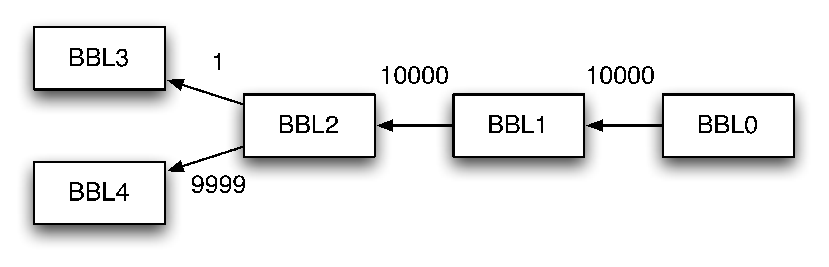
\includegraphics[width=0.64\linewidth]{figs/cfg0.eps}
    \caption{Example control flow graph. Nodes represent basic blocks and edges
    are control transfers. During dynamic profiling, we count how many times
    each edge is followed (edge labels). \label{fig:cfg0}}
\end{figure}


\subsubsection{Memory Integrity Tool (Memcheck)}

Memory integrity tools~\cite{memcheck, drmemory, asan} are designed to assist
developers by reporting (a) memory leakage errors implemented by instrumenting
known memory allocation and deallocation routines to check whether a program
exits having any allocated memory chunks not being deallocated and (b) usage of
uninitialized variable by tracking the propagations and usages of any
uninitialized variables throughout the program execution.
%
While it share much of its architectural characteristics with DFT as it tracks
the uninitialized memory entries using shadow memory area, it has its own
interpretations of general purpose instructions needed to perform tracking
operation.  Readers can notice that representative examples presented from
Table~\ref{tab:memcheck_tracking} are different from DFT interpretation in
Table~\ref{tab:dft_tracking}. And the checking operation (for the usage
uninitialized variables) is far more frequent in this case, as this is needed
for every instruction that has memory reference.

\begin{table}[h]
        \centering
\begin{tabular}{|l|l|}
\hline
{\bf Instruction} & {\bf Tag propagation rule} \\ \hline \hline
    {\tt \specialcell{ALU-OP OP1 $\leftarrow$ OP2 \\ (add, sub \dots)}} & 
    {\tt t(op1) $\vert=$ t(op2)}\\ \hline
    {\tt MOV OP1  $\leftarrow$  OP2} & {\tt t(op1) = t(op2)}     \\ \hline
    {\tt LOAD OP1 $\leftarrow$ [OP2]} & {\tt t(OP1) = t([OP2])}  \\ \hline
    {\tt STORE [OP1] $\leftarrow$ OP2} & {\tt t([OP1]) = t(OP2)} \\ \hline
\end{tabular}
\caption{presents an interpretation of DFT semantics for pseudo instruction set
architecture.}
\label{tab:memcheck_tracking}
\end{table}

To extend \sreplica to support a tool of the kind, we have to modify its core
components  that (a) translate {\tt x86} instructions into \tfa representation,
(b) perform optimization and so on. Even though we do not make fundamental
changes to its architecture, we still do not have clear understandings about
how system behaviors would change in respond as well as how frequent checking
operations of the tool would have impact.

\subsection{Instrumentation Infrastructure Study}
\label{ssec:inst_infra}

As we have discussed from Section~\ref{ssec:prev_eval}, the cost to instrument
event collect to the application thread accounts for large portion of its
runtime slowdown. In this section, we discuss about available considerations to
replace this substrate for performance improvement. First, we compare three
different DBI implementations including one that we use for \sreplica (PIN DBI)
and then talk about approaches of different categories based on binary writing
and hardware assistance.

\subsubsection{DBI Study} 
\label{ssec:dbi_study}

Dynamic binary instrumentation(DBI) frameworks enable the development of
program analysis tools for unknown binary by facilitating automatic low-level
instrumentation. This technology takes advantage of the process-level
virtualization populating the code cache entries that combines original codes
with users-authored analysis logics. This technique has become essential
building blocks in developing tools that enhance the security and reliability
of software systems.  Representative DBI frameworks for these are PIN~\cite{},
Valgrind~\cite{}, and DynamoRIO~\cite{}.
%
Forming a same layer between a running application and underlying operating
system, each framework comes with different capabilities and performance
implications as each framework’s design principles varies up to their major
target applications. However, developers who want to leverage the technology
were rarely informed regarding how to choose a framework that meets their
developmental requirements.
%
In this part, we compare three aforementioned frameworks by carefully examining
three different aspects – efficiency, capability, and usability. Purpose of our
work is to provide a proper guideline to developers who want to develop
security analysis tools enhancing this technology.

\subsubsection{Alternative Instrumentation Approaches}

\jikk{AWK}Trade-off for flexibility in DBI instrumentation, we need to pay high
overhead due to process level virtualization. Having this in mind, we want to
explore possible alternatives that can replace the substrate. Now, we are
looking at solutions based on {\it binary re-writing}~\cite{cfi, rewriting} and
instrumentation approach leveraging {\it DTrace}~\cite{} technology.

\subsubsection{Hardware Assisted Decoupled Analysis} 
\label{}

We are also considering to hardware based instrumentation to enhance
\sreplica's execution model. XXX \etal already proposed log based architecture
(LBA)~\cite{lba}, a framework for decoupled analysis having hardware level
support, but it suffered from too much amount of information collected from the
application and transferred using shared cache connecting two different cores.
%
Addressing the issue of communication volume and frequency with \sreplica's
capability in optimizing and reducing the amount of such informations by having
static off-line analysis, we also want to build a CPU extension that would
accelerate decoupled analysis. 
%
The main design and implementation challenges are (a) space requirement for
addition hardware need to be minimal and (b) the support should be flexible so
it can dynamically adopt to monitoring logics and support different kinds of
inline monitors.

\subsection{Overhead Modeling Framework}

\begin{figure}[tb]
    \centering
    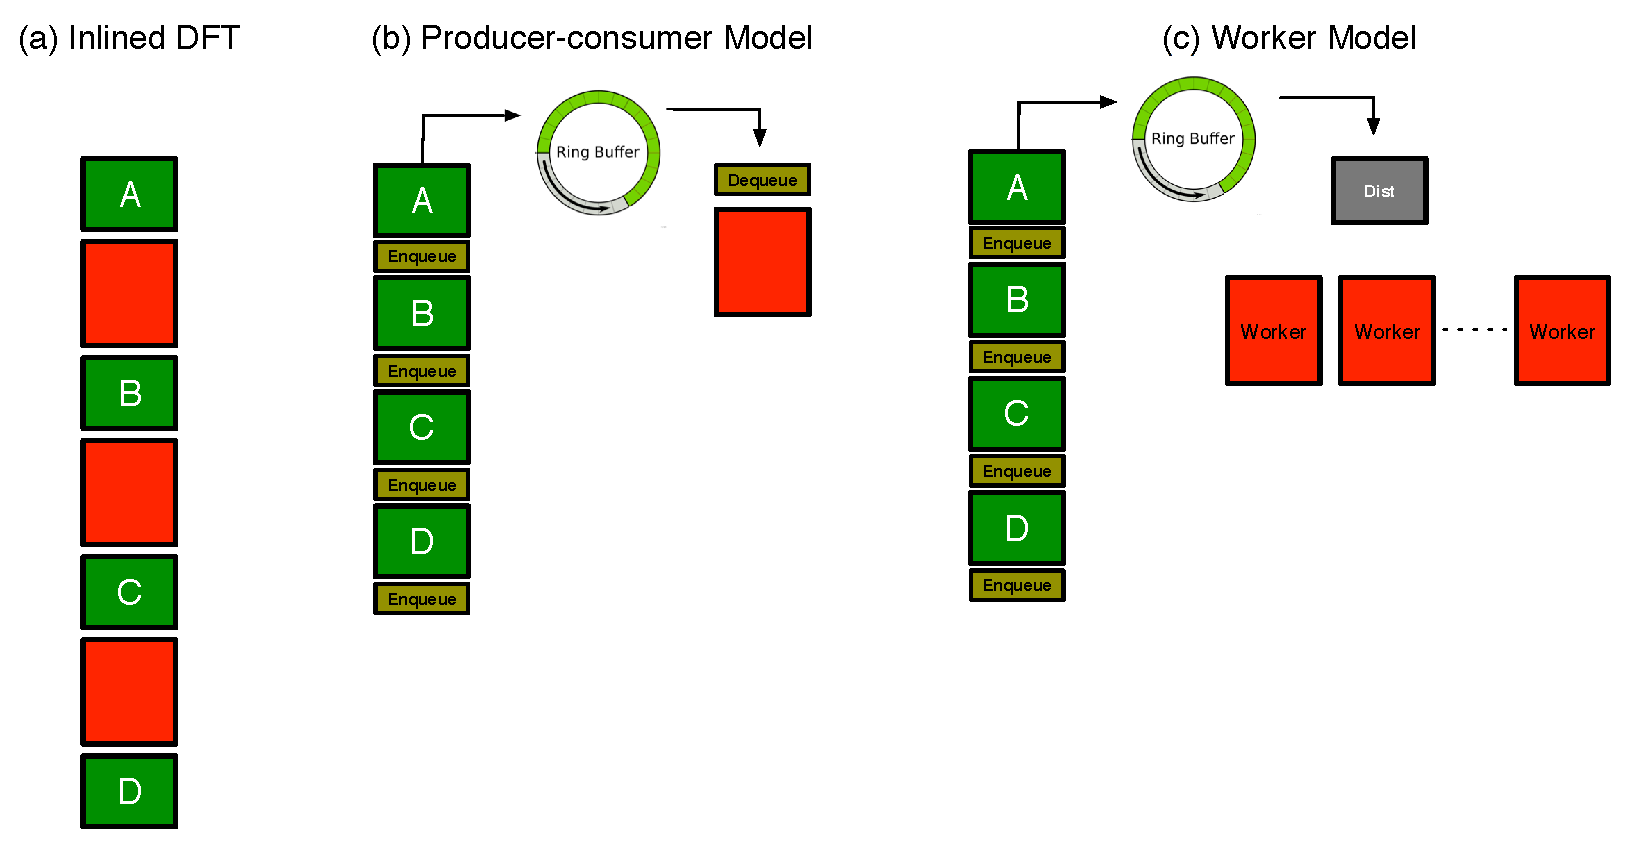
\includegraphics[width=0.90\linewidth]{figs/model0.eps}

    \caption{present three different models to instrument inline monitors. From
    the left to right it has (a) inlining model, (b) a producer - a consumer
    model, and (c) one producer - multiple consumers model.\label{fig:model0}}

\end{figure}

\subsubsection{Inlining Model}
\subsubsection{Producer-consumer Model}
\subsubsection{Worker poll Model}

